\chapter{Domain Name System}
\section{Overview}
This section will describe the technological fundamentals of DNS, as well as related technologies like IP addressing. The technologies will be described along with example software used to display different parts of the theory.

The section will also contain a description of the BIND DNS software, along with installation and user guide. 

This section will not focus on the chosen real-life case. This is a general description of the technology.
\section{IP Addressing}
\subsection{IP overview}
To access any resource on the internet (or LAN), be it a website or a specific device, a location is needed. When dealing with internet-related technologies, this location is specified by an \textit{IP address}. 

On any given network, an IP address should be unique to a specific device/server. However, local network routers generally have a private block of IP addresses for devices on that specific sub-net and a separate IP for the outside world (access to sub-net devices are forwarded to the specific devices by the router).
The router then acts as the \textit{gateway} to the outside world and should be accessible by an IP within the range of the sub-net.

To check the IP address of a device, the tool ifconfig (Linux) or ipconfig (windows) can be used

%\begin{figure}[h!]
%  \caption{A picture of a gull.}
%  \centering

\begin{figure}[h!]
	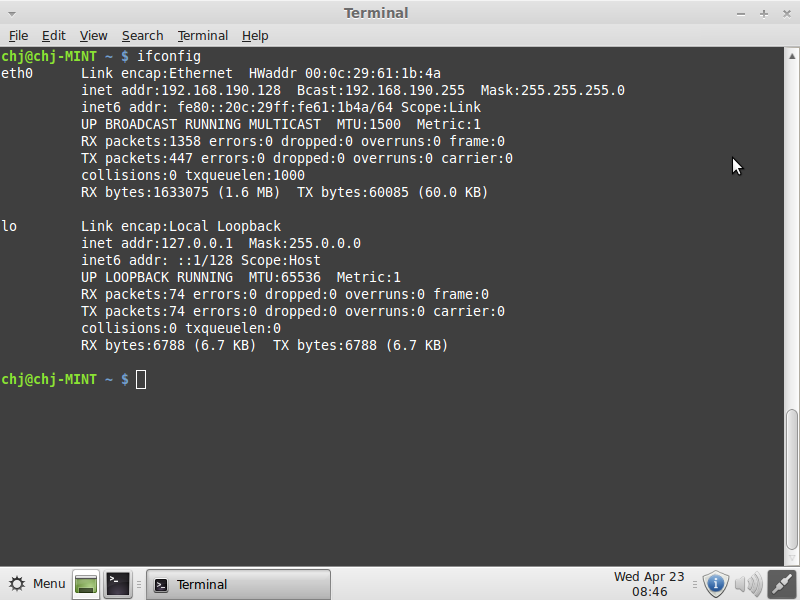
\includegraphics[width=\textwidth]{ifconfig.png}
\end{figure}


If the tool \textit{nm-tool} is run (on a Linux machine) the output will look like this:

[Insert picture of nm-tool]

Where 

\textbf{Address} 
Denotes the machines' IP on the local sub-net. Other devices on the sub-net will use this IP on to communicate with the device.

\textbf{Prefix} 
Denotes the 

%\textbf{IP versions}
\subsection{Checking IP and related}
How to check IP (Linux) ifconfig

nm-tool

%To understand DNS, you must understand IP addresses! [Altså Excercise 1!]
%Helt overordnet, hvad er det?
\section{Name Resolution and forwarding}
%Hvad er formålet med name resolution? Hvad gør det? Hvad får vi ud af det?
\subsection{Iterative}
\subsection{Recursive}
\subsection{Caching}
\subsection{Security [DNSSEC]}
\section{BIND}
\subsection{Downloading}
\subsection{Configuration}
\subsection{Basic Use}

%This chapter should contain an in-depth description of the technology,
%i.e. DNS, DDS, or RMI. You should at least address
%\begin{itemize}
%\item The purpose of the technology
%\item Technology alternatives
%\item Downloading, installing, configuring, and employing the technology
%\end{itemize}
